\documentclass[11pt, landscape]{article}

\usepackage[hmargin=1.25cm, vmargin=1.5cm]{geometry} % Document margins

\usepackage{amsmath}
\usepackage{amsthm}
\usepackage{graphicx}
\usepackage{mathtools}
\usepackage{fullpage}
\usepackage{verbatim}

\title{Brownian Dynein Model}

\newcommand{\mn}{\scalebox{0.7}[1.0]{-}}

\begin{document}

\maketitle

{\huge Bothbound Solution} \\
We now do a similar solution for velocities in the case where both of the model's binding domains are stuck to the microtubule.

\begin{figure}[h!]
  \caption{Key lengths and angles in bothbound dynein model.}
  \centering
    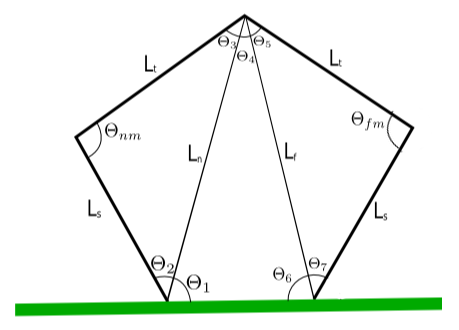
\includegraphics[width=0.7\textwidth]{../figures/bothbound_model.png}
\end{figure}

\section{Cartesian Coordinate Derivation}

By the law of cosines:
\begin{align}
  L_n &= \sqrt{L_{s}^2+L_{t}^2-2L_{t}L_{s}\cos(\Theta_{nm})}\\
  L_f &= \sqrt{L_{s}^2+L_{t}^2-2L_{t}L_{s}\cos(\Theta_{fm})}\\
\end{align}

By the law of cosines, we see that:
\begin{align}
  \Theta_{1} &= \cos^{-1}\bigg(\frac{L^2+L_{n}^2-L_{f}^2}{2LL_{n}}\bigg) \\
  \Theta_{2} &= \pm\cos^{-1}\bigg(\frac{L_{s}^2+L_{n}^2-L_{t}^2}{2L_{s}L_{n}}\bigg) \\
\end{align}

We use the following relations in the derivation:

\begin{align}
  \cos(\cos^{-1}(a) \pm \cos^{-1}(b)) &= ab \mp \sqrt{1-a^2}\sqrt{1-b^2}\\
  \sin(\cos^{-1}(a) \pm \cos^{-1}(b)) &= b\sqrt{1-a^2} \pm a\sqrt{1-b^2}\\
\end{align}

\subsection{Solving for $X_{nm}$ and $Y_{nm}$}

\begin{align}
  X_{nm} &= L_s\cos(\theta_1 + \theta_2)\\
  &= L_s\cos\left(\cos^{-1}\bigg(\frac{L^2+L_{n}^2-L_{f}^2}{2LL_{n}}\bigg) \pm\cos^{-1}\bigg(\frac{L_{s}^2+L_{n}^2-L_{t}^2}{2L_{s}L_{n}}\bigg)\right)\\
  &= L_s\left(\left(\frac{L^2+L_{n}^2-L_{f}^2}{2LL_{n}}\right)\left(\frac{L_{s}^2+L_{n}^2-L_{t}^2}{2L_{s}L_{n}}\right) \mp \sqrt{1-\left(\frac{L^2+L_{n}^2-L_{f}^2}{2LL_{n}}\right)^2}\sqrt{1-\left(\frac{L_{s}^2+L_{n}^2-L_{t}^2}{2L_{s}L_{n}}\right)^2}\right)\\
  &= L_{s}\Bigg( \Big(\frac{L^2+L_{n}^2-L_{f}^2}{2LL_{n}}\Big)\Big(\frac{L_{s}^2+L_{n}^2-L_{t}^2}{2L_{s}L_{n}}\Big) \mp \sqrt{1-\bigg(\frac{L^2+L_{n}^2-L_{f}^2}{2LL_{n}}\bigg)^2}\sqrt{1-\bigg(\frac{L_{s}^2+L_{n}^2-L_{t}^2}{2L_{s}L_{n}}\bigg)^2} \Bigg)\\
\end{align}

\begin{align}
  Y_{nm} &= L_s\sin(\theta_1 + \theta_2)\\
  &= L_s\left(\frac{L_{s}^2+L_{n}^2-L_{t}^2}{2L_{s}L_{n}}\right)\sqrt{1-\left(\frac{L^2+L_{n}^2-L_{f}^2}{2LL_{n}}\right)^2} \pm \left(\frac{L^2+L_{n}^2-L_{f}^2}{2LL_{n}}\right)\sqrt{1-\left(\frac{L_{s}^2+L_{n}^2-L_{t}^2}{2L_{s}L_{n}}\right)^2}\\
  &= L_{s}\Bigg(\frac{L_{s}^2+L_{n}^2-L_{t}^2}{2L_{s}L_{n}}\sqrt{1-\bigg(\frac{L^2+L_{n}^2-L_{f}^2}{2LL_{n}}\bigg)^2} \pm \frac{L^2+L_{n}^2-L_{f}^2}{2LL_{n}}\sqrt{1-\bigg(\frac{L_{s}^2+L_{n}^2-L_{t}^2}{2L_{s}L_{n}}\bigg)^2} \Bigg)\\
\end{align}

\end{document}
